\part{Background}
\chapter{Quantum Adiabaticity}\label{chap:2_adiabaticity}

\epigraph{I saw this movie about a bus that had to SPEED around a city, keeping its SPEED over fifty, and if its SPEED dropped, it would explode! I think it was called `The Bus That Couldn’t Slow Down'.}{Homer Simpson}

    
The concept of quantum adiabaticity is the central starting point of the work presented in this thesis. While in classical thermodynamics, an adiabatic process is essentially one where no heat or mass is transferred between a system and its environment, the quantum adiabatic theorem concerns itself more with the speed at which changes in a system Hamiltonian occur. The quantum adiabatic theorem, which I will explore in more detail in this chapter, states that \reminder{finish this}
        
    \section{The quantum adiabatic theorem}\label{sec:2.1_adiabatic_theorem}
    
    Imagine a quantum system that begins in the non-degenerate ground state of a time-dependent Hamiltonian. According to the the quantum adiabatic theorem, it will \emph{remain} in the instantaneous ground state provided the Hamiltonian changes sufficiently slowly. To take an intuitive example, we can consider a spin in a magnetic field that is rotated from the $x$ direction to the $z$ direction during some total time $\tau$. The Hamiltonian might be written as:
    \begin{equation}\label{eq:rotating_spin_H}
        H(t) = -\cos\Big(\frac{\pi t}{2 \tau}\Big)\sx - \sin \Big(\frac{\pi t}{2 \tau}\Big)\sz,
    \end{equation}
    where $\sx$ and $\sz$ are the Pauli matrices:
    \begin{equation}
        \sx = \mqty(0 & 1 \\ 1 & 0), \quad \sz = \mqty(1 & 0 \\ 0 & -1).  
    \end{equation}
    If the spin starts in the ground state of $H(0)$ (pointing in the $x$ direction, $\ket{\psi(0)} = \ket{+}$), then as the magnetic field is rotated, the spin starts precessing about the new direction of the field. This moves the spin toward the $z$ axis but also produces a component out of the $xz$ plane. As the total time for the rotation gets longer (\@i.e. the rotation gets slower compared to the precession), the state maintains a tighter and tighter orbit around the field direction. In the limit of $\tau \rightarrow \infty$, the state of the spin tracks the magnetic field perfectly, always in the ground state of $H(t)$ for all $t$. This is illustrated in Fig.~\ref{fig:bloch_rotating_spin} below, which shows the evolution of the system for increasing $\tau$ (and thus decreasing speed).
    
    \begin{figure}[h]
    \centering
    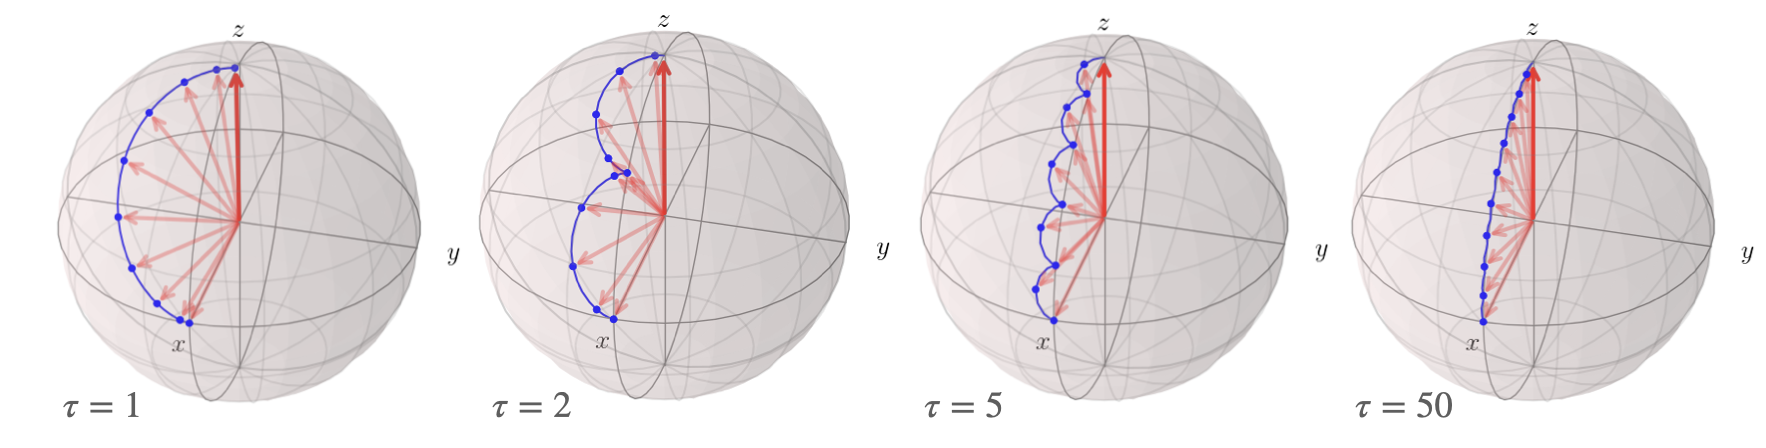
\includegraphics[width=0.9\linewidth]{images/magnetic_field_spin.png} \caption{Bloch sphere illustration of the single-spin system driven by the Hamiltonian of Eq.~\eqref{eq:rotating_spin_H} for different total driving times $\tau$.}\label{fig:bloch_rotating_spin}
    \end{figure}

    \subsection{Proof of the adiabatic theorem}\label{sec:2.1.1_proof_adiabatic_theorem}

    The above example gives some intuition for the behaviour of quantum systems as the time of evolution is slowed down, but it doesn't quite answer the question of what it means to be `slow enough' in the general case, ~\@i.e. what one would refer to as the \emph{adiabatic condition}. In order to characterise this regime, we first imagine a state $\psi(t)$ which evolves under some time-dependent Hamiltonian $H(t)$. For convenience, we redefine time through the parameter $\lambda = \frac{t}{\tau} \in [0,1]$, such that $\psi(t), H(t) \rightarrow \psi(\lambda), H(\lambda)$ vary smoothly as a function of $\lambda$. This is often done to capture the fact that there may be a natural parameterisation of the changing Hamiltonian such as, for example, two different angles describing a varying magnetic field, which we may want to explore. The parameter space we build generally has some geometric properties that relate to non-adiabatic effects, so it becomes important to talk about these abstract parameters instead of time. But more on this later!
    
    For each value of $\lambda$ throughout the evolution, we have a time-independent `instantaneous' Hamiltonian which can be diagonalised:
    \begin{equation}\label{eq:instantaneous_schroedinger}
        H(\lambda)\ket{n(\lambda)} = E_n(\lambda)\ket{n(\lambda)},
    \end{equation}
    where $E_n(\lambda)$ are the eigenenergies and $\ket{n(\lambda)}$ are the eigenvectors. Note that this is \emph{not} the time-dependent solution. The vectors $\ket{n(\lambda)}$ constitute a basis, so we can expand our quantum state at any value of $\lambda$ as:
    \begin{equation}\label{eq:adiabatic_basis_expansion}
        \ket{\psi(\lambda)} = \sum_n c_n(\lambda)e^{i \tau \theta_n(\lambda)}\ket{n(\lambda)},
    \end{equation}
    where $c(\lambda)$ are time-dependent coefficients through the parameter $\lambda$ and $e^{i \tau \theta_n(\lambda)}$ is the phase factor that an eigenstate picks up as a consequence of time-evolution with a time-independent Hamiltonian:
    \begin{equation}\label{eq:dynamical_phase}
        \theta_n(\lambda) = -\frac{1}{\hbar} \int_0^{\lambda} E_n(\lambda') d\lambda'.
    \end{equation}
    The factor of $\tau$ is simply a consequence of the change in variables $t \rightarrow \lambda$, since $\frac{d \lambda}{dt} = \dotlambda = \frac{1}{\tau}$.
    
    Thus, the task is now to solve the time-dependent Schr\"{o}dinger equation:
    \begin{equation}\label{eq:td-schroedinger}
        i\hbar \dotlambda \ket{\dlambda \psi(\lambda)} = H(\lambda) \ket{\psi(\lambda)},
    \end{equation}
    where $\dlambda$ is the partial derivative with respect to the parameter $\lambda$. We can then use the expansion Eq.~\eqref{eq:adiabatic_basis_expansion}, differentiate and take the inner product with some eigenstate $\bra{m(\lambda)}$ to get:
    \begin{equation}\label{eq:adiabatic_derivation}
        \begin{aligned}
         \frac{i\hbar}{\tau} \dlambda \sum_n c_n e^{i \tau \theta_n} \ket{n} &= H \sum_n c_n e^{i \tau \theta_n} \ket{n} \\
        \sum_n \Big( \dlambda c_n \ket{n} + c_n \ket{\dlambda n} + i \tau \dlambda\theta_n c_n \ket{n} \Big)e^{i \tau \theta_n} &= -\frac{i \tau}{\hbar} \sum_n E_n c_n e^{i \tau \theta_n} \ket{n} \\
        \sum_n \Big( \dlambda c_n \ket{n} + c_n \ket{\dlambda n} \Big)e^{i \tau \theta_n} &= 0 \\
        \dlambda c_m  &= - \sum_n c_n \braket{m}{\dlambda n}e^{i\tau(\theta_n-\theta_m)}
        \end{aligned}
    \end{equation}
    where the last two lines are a consequence of the fact that $i \tau \dlambda \theta_n(\lambda) = -\frac{i \tau}{\hbar} E_n(\lambda)$ and the the orthogonality of $\ket{m}$ and $\ket{n}$ when $m \neq n$. Note that I have removed the explicit dependence on $\lambda$ for the sake of readability and to make writing this all out more bearable and I will continue with this convention for the rest of the chapter unless otherwise stated. 
    
    The above differential equation is exact and describes the evolution of the coefficients $c_n$,  but it doesn't give much of a clue as to what `slow' time evolution means with respect to the changes in the Hamiltonian. For that, we can express the term $\braket{m}{\dlambda n}$ in terms of the changing Hamiltonian. This is done by differentiating Eq.~\eqref{eq:instantaneous_schroedinger} and then again taking the inner product with $\bra{m}$ to get:
    \begin{equation}\label{eq:hamiltonian_derivative}
        \begin{aligned}
            \dotlambda \Big(\dlambda{H}\ket{n} + H \ket{\dlambda n}\Big)  &= \dotlambda \Big(\dlambda{E_n}\ket{n} + E_n \ket{\dlambda n}\Big) \\
            \mel{m}{\dlambda H}{n} + \mel{m}{H}{\dlambda n} &= \dlambda E_n\braket{m}{n} + E_n \braket{m}{\dlambda n} \\
            E_m \braket{m}{\dlambda n} - E_n \braket{m}{\dlambda n} &= - \mel{m}{\dlambda H}{n} \\
            \braket{m}{\dlambda n} &= - \frac{\mel{m}{\dlambda H}{n}}{E_m - E_n}, \quad m \neq n
        \end{aligned}
    \end{equation}
    
    What the last line in Eq.~\eqref{eq:hamiltonian_derivative} shows is that we can express the term $\braket{m}{\dlambda n}$ in terms of the matrix components of $\dlambda H$ and the energy gap between the two eigenstates. If we plug this back into the final line of Eq.~\eqref{eq:adiabatic_derivation}, we find that:
    \begin{equation}\label{eq:coefficient_exact}
            \dlambda c_m -  c_m \braket{m}{\dlambda m} = \sum_{n \neq m} c_n  \frac{\mel{m}{\dlambda H}{n}}{E_m - E_n}e^{i \tau (\theta_n-\theta_m)}.
    \end{equation}
    When the term on the RHS is small we can neglect it and the solution for the remaining differential equation of $c_m$ is just:
    \begin{equation}\label{eq:c_adiabatic}
        c_m(\lambda) = c_m(0)e^{i \gamma_m(\lambda)},
    \end{equation}
    where:
    \begin{equation}\label{eq:geometric_phase}
        \gamma_m(\lambda) = i \int_0^{\lambda} \braket{m}{\partial_{\lambda'} m} d \lambda' 
    \end{equation}
    is the geometric (or Berry) phase \cite{pancharatnam_generalized_1956, longuet-higgins_studies_1958, berry_quantal_1984}. It arises from the fact that if the Hamiltonian varies according to $\lambda$ in a closed loop way, \@~i.e. it returns to its starting point at the end of the evolution, the wavefunction might not. Think Foucault's pendulum, which changes its plane of swinging due to the Earth's rotation around its own axis and does not necessarily return to its initial state after a full rotation! Both the appearance of the geometric phase in Eq.~\eqref{eq:c_adiabatic} and the changing plane of Foucault's pendulum are consequences of the geometry or `curvature' of the parameter space in which the dynamics occur and are related to concepts like parallel transport. \reminder{does this need citations? More elaboration?} 

    The constraint that the RHS of Eq.~\eqref{eq:coefficient_exact} be negligible is exactly the adiabatic condition, which can be seen by checking that $\abs{c_m(\lambda)}^2 = \abs{c_m(0)}^2$ in Eq.~\eqref{eq:c_adiabatic}. What this means is that a state starting in a particular eigenstate $\ket{m(\lambda)}$ will remain in that state under these circumstances, ~\@e.g. for $c_m(0) = 1$ and $c_{m \neq n}(0) = 0$:
    \begin{equation}\label{eq:adiabatic_states}
        \ket{\psi(\lambda)} = e^{i \tau \theta_m(\lambda)}e^{i \gamma_m(\lambda)} \ket{m(\lambda)}
    \end{equation}
    the $m^{\text{th}}$ eigenstate stays in the $m^{\text{th}}$ eigenstate.
    
    So to understand adiabaticity, we need to understand what conditions lead to the case where
    \begin{equation}\label{eq:adiabaticity_condition}
        \sum_{n \neq m} c_n \frac{\mel{m}{\dlambda H}{n}}{E_m - E_n}e^{i \tau (\theta_n-\theta_m)} \ll 1,
    \end{equation}
    which is exactly what the next section sets out to do.
    
    \subsection{The adiabatic condition: how slow is \emph{slow}?}\label{sec:2.1.2_adiabatic_condition}

    The condition given by Eq.~\eqref{eq:adiabaticity_condition} contains terms relating both to the rate of change of the Hamiltonian with respect to $\lambda$ (expressed in terms of matrix elements $\mel{m}{\dlambda H}{n}$) and the energy gap between eigenstates $E_m - E_n$. It is not too hard to see that when the energy gaps are very large, these terms can be neglected. However, let us try to derive a more concrete and quantitative measure for `slowness'.

    First, we can go back to the intermediate result from Eq.~\eqref{eq:coefficient_exact} and write it out as:
    \begin{equation}\label{eq:perturbative_adiabatic}
        \dlambda c_m = \sum_k c_k \frac{\mel{m}{\dlambda H}{k}}{E_m - E_k} e^{-\frac{i \tau}{\hbar}\int_0^{\lambda} E_m(\lambda') - E_k(\lambda') d\lambda'},
    \end{equation}
    where the exponential at the end is just a the dynamical phase from Eq.~\eqref{eq:dynamical_phase}. Let's again take the case that $c_n(\lambda) = 1$ and $c_{m \neq n}(\lambda) = 0$ at all values of $\lambda$, the approximate adiabatic solution. This leaves us with an equation which can be integrated:
    \begin{equation}\label{eq:nonadiabatic_perturbation}
        \begin{aligned}
            \dlambda c_{m \neq n} &= \frac{\mel{m}{\dlambda H}{n}}{E_m - E_n} e^{-\frac{i \tau }{\hbar}\int_0^{\lambda} E_m(\lambda') - E_n(\lambda') d\lambda'} \\
            \rightarrow c_{m \neq n} (1) &= \int_0^1 \frac{\mel{m}{\dlambda H}{n}}{E_m(\lambda) - E_n(\lambda)} e^{-\frac{i \tau }{\hbar}\int_0^{\lambda} E_m(\lambda') - E_n(\lambda') d\lambda'} d\lambda,
        \end{aligned}
    \end{equation}
    where, as already stated more than enough times, we expect the quantity $c_{m \neq n}$ to be $0$ (or as close to it as possible) for the adiabatic condition to hold. In fact, this was an assumption in the previous simplifying step! You can view these coefficients as the probabilities of transitioning out of the eigenstate $\ket{m}$ to the eigenstate $\ket{n}$ throughout the evolution. Since we'd like to keep our system in its initial (in this case $\ket{m}$) eigenstate at all times, it makes sense to minimise the RHS of Eq.~\eqref{eq:nonadiabatic_perturbation}. So, let us simplify the problem by first considering what are the quantities we can bound and where the largest contributions come from. In the case of the rate of change of the Hamiltonian, the largest matrix element will contribute more than the rest, so we can upper bound the contribution to the error via:
    \begin{equation}\label{eq:max_matrix_el}
        \max_{\ket{n(\lambda)}}\Big({\mel{m(\lambda)}{\dlambda H(\lambda)}{n(\lambda)}}\Big) \approx \overline{\mel{m}{\dlambda H}{n}}.
    \end{equation}
    The energy difference between the eigenstates in the denominator will have the largest impact when it is minimised (bearing in mind that this quantity is undefined if the two states are degenerate), so we can take the minimum possible energy gap as:
    \begin{equation}\label{eq:min_energy_diff}
        \min_{E_n(\lambda)} \Big(E_m(\lambda) - E_n(\lambda)\Big) = \overline{E_m - E_n}.
    \end{equation}
    With these two quantities in mind, we can now evaluate the last line of Eq.~\eqref{eq:nonadiabatic_perturbation} to find:
    \begin{equation}\label{eq:deriving_adiabatic_condition_final}
        \begin{aligned}
            c_{m \neq n} (1) &\approx \frac{\overline{\mel{m}{\dlambda H}{n}}}{\overline{E_m - E_n}} \int_0^1 e^{\frac{i \tau }{\hbar} \overline{E_m - E_n} \lambda} d \lambda \\
            &= \frac{i \hbar \overline{\mel{m}{\dlambda H}{n}}}{\tau(\overline{E_m - E_n})^2} \Big(e^{-\frac{i \tau }{\hbar}\overline{E_m - E_n}} - 1 \Big) \\
            &\approx \frac{i \hbar \dotlambda \overline{\mel{m}{\dlambda H}{n}}}{(\overline{E_m - E_n})^2},
        \end{aligned}
    \end{equation}
    where the final simplification is just due to the fact that the exponential term is oscillating with a maximum value of $1$. Since our goal is to bound $c_{m \neq n} (1)$ from above, we'll just set it to that maximum value. This leaves us with the simple criterion of what `slow' means with respect to the adiabatic regime:
    \begin{equation}\label{eq:adiabatic_criterion}
        \frac{i \hbar \dotlambda \overline{\mel{m}{\dlambda H}{n}}}{(\overline{E_m - E_n})^2} \ll 1, \quad m \neq n.
    \end{equation}

    In the example Hamiltonian of Eq.~\eqref{eq:rotating_spin_H}, the energy gap between its two eigenstates $\ket{\psi_1(t)}$ and $\ket{\psi_2(t)}$ is a constant: $E_{\psi_1} - E_{\psi_2} = 2$, and so are the matrix elements $\mel{\psi_1}{\dot{H}}{\psi_2} = \mel{\psi_2}{\dot{H}}{\psi_1} = \frac{\pi}{2 \tau}$. The dependence on $\tau$ of the off-diagonal matrix elements of $\dot{H}$ make the results of Fig.~\ref{fig:bloch_rotating_spin} immediately clearer: as $\tau$ increases (and hence the evolution is slower), the non-adiabatic component of Eq.~\eqref{eq:adiabatic_criterion} decreases proportionately to it. 

    I chose to elaborate on this proof in particular because it gave me a lot of intuition for what the adiabatic theorem \emph{is} and what I should look out for when I think of `slow' processes. In practice, however, it is not immediately obvious how the quantity stated in Eq.~\eqref{eq:adiabatic_criterion} relates to, say, the fidelity of the final state with respect to the desired state or how large $\tau$, the evolution time, has to be in order to lead to a fidelity of some magnitude. While it is possible to find these bounds, the proof is quite lengthy and not necessary for the purposes of this thesis, so instead I will refer you to \cite{reichardt_quantum_2004, childs_lecture_2008} for more details.
    
    \section{The adiabatic gauge potential}\label{sec:2.2_AGP}

    The previous section introduced quantum adiabaticity and presented some intuition for what non-adiabatic effects look like at fast driving times. In this section, I want to establish the deeply related concept of the adiabatic gauge potential (\acrref{AGP}) \cite{kolodrubetz_geometry_2017}, a key player in the subject matter of this thesis and a fascinating mathematical object in its own right. While the \acrref{AGP} has primarily been studied in the context of suppressing non-adiabatic effects \cite{sels_minimizing_2017, claeys_floquet-engineering_2019}, as will be its central role in this thesis, in recent years it has also been shown to be a potential probe for quantum chaos \cite{pandey_adiabatic_2020} and has been proposed for the study of thermalisation \cite{nandy_delayed_2022}. \reminder{add more here, mention ``geometric in nature"}

    \subsection{The moving frame Hamiltonian}

    In Section \ref{sec:2.1.1_proof_adiabatic_theorem} I spent a lot of time working in the instantaneous eigenbasis of the Hamiltonian where it is diagonalised, à la Eq.~\eqref{eq:instantaneous_schroedinger}. For a general Hamiltonian, it is possible to go to this `moving frame' picture by rotating the Hamiltonian via some unitary $U$ so that it becomes diagonal at each point in time. If we start with some arbitrary Hamiltonian $H(\lambda)$ in some sort of lab frame' that depends on time through the parameter(s) $\lambda(t)$, it can be diagonalised through $\Tilde{H} = U^{\dagger}(\lambda)H(\lambda)U(\lambda)$, where the $\sim$ implies that we are now in the basis of the moving frame and that the Hamiltonian is diagonal. In general, whenever the tilde symbol appears above an operator throughout this section, all it means is that we are working in this new basis: $\Tilde{\sigma} = \adj{U}\sigma U$.

    We can also view the quantum system evolving under the Hamiltonian in this moving frame picture: $\ket*{\Tilde{\psi}} = U^{\dagger}\ket{\psi}$, which is like expanding the wave function in the moving frame (or instantaneous) basis exactly as was done in Eq.~\eqref{eq:adiabatic_basis_expansion}. Given this new viewpoint, trying to solve the Schr\"{o}dinger equation, this time with the operators explicitly in mind, reveals something interesting:
    \begin{equation}\label{eq:moving_frame_schrodinger}
        \begin{aligned}
            i \hbar \frac{d \ket*{\Tilde{\psi}}}{dt} &= i \hbar \Big( \frac{d \adj{U}}{dt}\ket*{\psi} + \adj{U} \frac{d \ket{\psi}}{dt} \Big) \\
            &= i \hbar \dotlambda \frac{\partial \adj{U}}{\partial \lambda}\ket{\psi} + \adj{U} H\ket{\psi}\\
            &= \dotlambda \Big(i\hbar \frac{\partial \adj{U}}{\partial \lambda}U \Big)\ket*{\Tilde{\psi}} + \adj{U} H U \ket*{\Tilde{\psi}} \\
            &= \Big(\Tilde{H} - \dotlambda\Tilde{\AGP{\lambda}}\Big) \ket*{\Tilde{\psi}},
        \end{aligned}
    \end{equation}
    where the operator $\Tilde{\AGP{\lambda}}$ is the \emph{adiabatic gauge potential} with respect to the parameter $\lambda$ in the moving frame of the Hamiltonian $H$ and is expressed as:
    \begin{equation}\label{eq:AGP_in_terms_of_U}
        \Tilde{\AGP{\lambda}} = i\hbar \adj{U}\dlambda U.
    \end{equation}
    The name `gauge potential' generally refers to operators that are generators of continuous unitary translations in parameter space \cite{kolodrubetz_geometry_2017} of some unitary transformation $U$ and generally takes the form of a derivative operator. While there are many such gauge potentials out there, we'll restrict ourselves to the specific case of adiabaticity where the transformation $U(\lambda)$ explicitly takes a wavefunction in an arbitrary basis to the adiabatic or instantaneous basis. 
    
    So what we find is that the wavefunction in the moving frame basis evolves under a combination of the diagonal component $\Tilde{H}$ and some additional term proportional both to the speed at which the parameter $\lambda$ varies and the \acrref{AGP}. At this point I want to note that while there are $\sim$ symbols all over the place, we can actually apply the inverse unitary operation in order to work back in lab frame basis: $\Tilde{H} - \dotlambda\Tilde{\AGP{\lambda}} \xrightarrow{U \{ \cdot \} \adj{U}} H - \dotlambda \AGP{\lambda}$. In fact, this transformation makes it easy to see how we can think of the AGP in the lab frame as nothing more than the derivative operator: $\AGP{\lambda} = i\hbar\dlambda$. 

    To see this, take any quantum state written in some basis, \@~e.g. $\ket{\psi} = \sum_n \psi_n \ket{n}$. Then in the moving frame basis we have:
    \begin{equation}\label{eq:AGP_basis_change}
            \ket{\psi} = \sum_n \psi_n \adj{U}(\lambda) \ket{n} = \sum_{\Tilde{n}} \Tilde{\psi}_n (\lambda) \ket*{\Tilde{n}(\lambda)},
    \end{equation}
    where $\Tilde{\psi}_n (\lambda) = \sum_n \adj{U}(\lambda) \psi_n = \braket{\Tilde{n}(\lambda)}{\psi}$ and the dependence on $\lambda$ enters into the basis vectors through the rotation $U(\lambda)$. These two bases can now allow us to look at the matrix elements of $\AGP{\lambda}$ in both:
    \begin{equation}\label{eq:AGP_as_derivative}
        \begin{aligned}
            \mel{n}{\Tilde{\AGP{\lambda}}}{m} &= \mel{n}{i\hbar \adj{U}\dlambda U}{m} \\
            &= i\hbar \mel{\Tilde{n}(\lambda)}{\dlambda}{\Tilde{m}(\lambda)} \\
            &= \mel{\Tilde{n}(\lambda)}{\AGP{\lambda}}{\Tilde{m}(\lambda)}
        \end{aligned}
    \end{equation}
    where the last line is simply the statement that in the lab frame $\AGP{\lambda} = i\hbar \dlambda$.

    \subsection{Matrix elements of the \acrref{AGP}}

    What I've shown you so far is that when we try to solve the Schr\"{o}dinger equation for a quantum system evolving under a time-dependent Hamiltonian in the basis of the `moving frame', \@~i.e. in the basis where the time-dependent Hamiltonian is diagonalised, we find that the evolution happens under a `decorated' Hamiltonian with an additional operator that I've dubbed the adiabatic gauge potential or \acrref{AGP}. We found that in the lab frame, it is the derivative operator with respect to the time-dependent parameters driving the Hamiltonian. What remains is to link this to our discussion of adiabaticity and the adiabatic condition of Section \ref{sec:2.1_adiabatic_theorem}.

    Let us return to the matrix elements of the lab frame \acrref{AGP} and see what they are in the adiabatic basis of Eq.~\eqref{eq:instantaneous_schroedinger}, which is the eigenbasis of the instantaneous Hamiltonian. The first thing that jumps out is that the diagonal elements of the \acrref{AGP} are very familiar:
    \begin{equation}\label{eq:AGP_diagonal}
        \mel{n(\lambda)}{\AGP{\lambda}}{n(\lambda)} = i\hbar \mel{n(\lambda)}{\dlambda}{n(\lambda)}.
    \end{equation}
    The terms on the RHS are something known as the Berry connections and they look familiar because they are the integrands of the geometric phase (Eq.~\eqref{eq:geometric_phase}) that we found when deriving the adiabatic condition! I mentioned that the geometric phase is related to the geometry or `curvature' of the parameter space of the adiabatic Hamiltonian and it turns out that the \acrref{AGP} contains information about this geometry. 

    In order to understand what the off-diagonal elements of the AGP are, we can make use of the fact that in the instantaneous Hamiltonian basis $\mel{m}{H}{n} = 0$ for $m \neq n$. Differentiating with respect to the parameter $\lambda$ gives:
    \begin{equation}\label{eq:differentiating_adiabatic_offdiagonals}
       \begin{aligned}
           \mel{\dlambda m}{H}{n} + \mel{n}{\dlambda H}{n} + \mel{n}{H}{\dlambda m} &= 0 \\
           E_n \braket{\dlambda m}{n} + E_m \braket{m}{\dlambda n} + \mel{n}{\dlambda H}{n} &= 0 \\
           (E_m - E_n) \braket{m}{\dlambda n} + \mel{n}{\dlambda H}{n} &= 0 \\
           \frac{-i}{\hbar} (E_m - E_n) \mel{m}{\AGP{\lambda}}{n} + \mel{n}{\dlambda H}{n} &= 0 \\
           \mel{m}{\AGP{\lambda}}{n} &= i\hbar \frac{\mel{m}{\dlambda H}{n}}{(E_n - E_m)}
       \end{aligned} 
    \end{equation}
    where I'll stress again that since we're working in the adiabatic basis, all eigenstates, eigenenergies and the operators depend on $\lambda$. The final line is familiar: the off-diagonal elements of the \acrref{AGP} are proportional to the non-adiabatic contribution we derived back in Eq.~\eqref{eq:deriving_adiabatic_condition_final}. The full operator in the adiabatic basis is:
    \begin{equation}\label{eq:AGP_adiabatic_basis}
        \AGP{\lambda} = i\hbar\Big(\sum_n \braket{n}{\dlambda n} \dyad{n} + \sum_{m \neq n} \ket{m} \frac{\mel{m}{\dlambda H}{n}}{(E_n - E_m)} \bra{n} \Big)
    \end{equation}

    The outcome of this section then, is the revelation that this (initially mysterious) operator known as the \acrref{AGP} is deeply linked to the notion of adiabaticity in quantum systems: its diagonal terms are related to the geometry of the parameter space of adiabatic dynamics while its off-diagonals elements describe the non-adiabatic effects experienced by a state when it is driven by a time-dependent Hamiltonian. It is useful to note that in the final line of Eq.~\eqref{eq:moving_frame_schrodinger} we found that the Schr\"{o}dinger equation corresponding to the evolution of the instantaneous eigenstates is:
    \begin{equation}\label{eq:schrodinger_moving_frame_2}
        i \hbar \frac{d \ket*{\Tilde{\psi}}}{dt} = \Big( \Tilde{H} - \dotlambda \AGP{\lambda} \Big) \ket*{\Tilde{\psi}},
    \end{equation}
    where now it is not difficult to find how each of these operators contributes to the results of Section \ref{sec:2.1.1_proof_adiabatic_theorem}. The moving frame or instantaneous Hamiltonian generates the dynamical phase factor in Eq.~\eqref{eq:dynamical_phase}, the diagonal elements of the \acrref{AGP} produce the geometric phase factor given by Eq.~\eqref{eq:geometric_phase} and the off-diagonal elements of \acrref{AGP} are responsible for the non-adiabatic transitions out of the eigenstates which we upper bounded in Section \ref{sec:2.1.2_adiabatic_condition}. For a more detailed proof of how to derive the adiabatic theorem starting from Eq.~\eqref{eq:schrodinger_moving_frame_2} I recommend \cite{petiziol_accelerated_2020}. \reminder{Shall I include the proof in the Appendix instead? It's quite long but maybe it's nice to have for a bit of context.}
    
    \section{Counterdiabatic Driving}\label{sec:2.3_CD}

    Having done all this work to characterise and understand the \acrref{AGP} and the adiabatic theorem, we now come to a very important question which defines just about the entirety of this thesis: \emph{why do we care}? What is it about adiabatic dynamics and quantifying non-adiabatic transformations and understanding what generates them important? The answer is simple: adiabatic processes are useful. The ability to drive a time-dependent Hamiltonian while remaining in a some eigenstate of the system is something that can be used to prepare interesting quantum states \cite{dimitrova_many-body_2022}, to solve combinatorics problems encoded in quantum systems \cite{ebadi_quantum_2022, pichler_quantum_2018} or even to synthesise effective ramps and quantum logic gates \cite{pelegri_high-fidelity_2022} among many other applications. 
    
    The most natural way of exploiting adiabatic protocols is by adhering to the adiabatic condition. However, as is often the case when it come to the control of quantum systems, things aren't quite that simple. In practice, in the average case changing a Hamiltonian slowly enough to satisfy Eq.~\eqref{eq:adiabatic_criterion} leads to the system being overwhelmed by decoherence. Furthermore, as system sizes get larger, the energy gaps between the instantaneous eigenstates tend to get smaller requiring slower and slower driving, making adiabatic protocols unscalable. The result, inevitably, is that we need to find ways to achieve the same results as adiabatic processes but without requiring the prohibitively long driving times that are demanded by Eq.~\eqref{eq:adiabatic_criterion}.
    
    Luckily, our analysis of the adiabatic condition and the \acrref{AGP} has given us a clue as to how we might be able to achieve fast driving without the eigenstate deformations that the adiabatic condition demands. Looking back at Eq.~\eqref{eq:schrodinger_moving_frame_2}, we might first note that our goal is to have the system follow the eigenstates of the instantaneous Hamiltonian and that in order to do this, we need to remove the $\dotlambda \AGP{\lambda}$ term. In fact, a very intuitive way to do this in practice would be simply to apply an additional operator which exactly cancels out the \acrref{AGP}:
    \begin{equation}
    	\Tilde{H}_{\rm effective} = \Tilde{H} - \dotlambda \AGP{\lambda} + \dotlambda \AGP{\lambda} = \Tilde{H}.
    \end{equation}
    This seems simple enough and in fact it is a thought 

    \begin{equation}\label{eq:CD_Hamiltonian}
    H_{CD}(\lambda) = H(\lambda) + \dotlambda \mathcal{A}_\lambda,
    \end{equation}

    \subsection{The problem: finding the \acrref{AGP}}

    \subsection{A classic(al) analogy: the waiter and the glass of water}

    I will take a brief detour away from all the mathematics involved in 
    
    \subsection{Transitionless Driving}
    The form of the dynamical Hamiltonian enforcing this is \cite{berry_transitionless_2009}:
    \begin{equation}\label{eq:counterdiabatic}
        H_{\mathrm{CD}}(t) = H_0 (t) + i\hbar \sum_n (\ket{\partial_t n}\bra{n} - \bra{n}\ket{\partial_t n}\ket{n}\bra{n}),
    \end{equation}
    \subsection{Variational counterdiabatic driving}

    \begin{equation}\label{eq:energy_derivative}
        \begin{aligned}
            \frac{dE}{dt} &= \frac{d}{dt}\ev*{\Tilde{H}}{\Tilde{\psi}} \\
            &= \dotlambda \ev*{\dlambda \Tilde{H}}{\Tilde{\psi}} - \frac{i}{\hbar} \dotlambda \ev*{\comm*{\Tilde{\AGP{\lambda}}}{\Tilde{H}}}{\Tilde{\psi}} \\
            &= -\dotlambda F_{\lambda} - \frac{i}{\hbar} \dotlambda \ev{\comm{\AGP{\lambda}}{H}}{\psi},
        \end{aligned}
    \end{equation}
    where the commutator in the second line appears because $i\hbar d_t \ket*{\Tilde{\psi}} = (\Tilde{H} - \dotlambda\Tilde{\AGP{\lambda}}) \ket*{\Tilde{\psi}}$
    
    Following the methods of Ref.~\cite{sels_minimizing_2017}, the problem of finding the optimal adiabatic gauge potential can be cast as the minimisation of the Hilbert-Schmidt norm of the operators
    \begin{equation}\label{eq:Goperator}
     G_{\lambda}= \dlambda H_\beta + i\comm{\mathcal{A}_\lambda}{H_\beta},
    \end{equation}
    which is equivalent to minimisation of the action
    \begin{equation}\label{eq:actionCD}
    \mathcal{S}(\mathcal{A}_{\lambda}) = \Trace{\left[G_{\lambda}(\mathcal{A}_{\lambda})^2\right]},
    \end{equation}
    with respect to $\mathcal{A}_{\lambda}$.
    \subsection{Nested commutator expansion}
    \subsection{Krylov methods}

    \subsection{Shortcuts to adiabaticity}
    
    Here I'm going to talk about Shortcuts to Adiabaticity 
    (\acrref{STA})
